% AI Ops Assistant: short project presentation (build: pdflatex AI_Ops_Assistant.tex)
\documentclass[aspectratio=169,11pt]{beamer}
\usepackage[T1]{fontenc}
\usepackage[utf8]{inputenc}
\usepackage{tgheros}
\renewcommand{\familydefault}{\sfdefault}
\usepackage{graphicx}
\usepackage{booktabs}
\usepackage{array}
\usepackage{tikz}
\hypersetup{hidelinks,pdfstartview={}}
\graphicspath{{../images/}}
% No hyphenation: words are never split with a dash
\hyphenpenalty=10000
\exhyphenpenalty=10000
\tolerance=9999
\emergencystretch=3em

\definecolor{ink}{HTML}{1F2933}
\definecolor{muted}{HTML}{616E7C}
\definecolor{accent}{HTML}{C0392B}
\definecolor{calm}{HTML}{2C7BE5}
\definecolor{paper}{HTML}{FFFFFF}
\definecolor{soft}{HTML}{F3F5F7}

\setbeamertemplate{navigation symbols}{}
\setbeamercolor{background canvas}{bg=paper}
\setbeamercolor{normal text}{fg=ink}
\setbeamercolor{frametitle}{fg=ink}
\setbeamercolor{itemize item}{fg=accent}
\setbeamertemplate{itemize item}{\raisebox{0.15em}{\rule{0.4em}{0.4em}}}
\setbeamerfont{frametitle}{size=\Large,series=\bfseries}
\setbeamertemplate{frametitle}{\vspace{0.6em}\insertframetitle\par\vspace{0.1em}{\color{accent}\rule{2.2em}{2pt}}}
\setbeamertemplate{footline}{\hfill{\color{muted}\scriptsize AI Ops Assistant \quad \insertframenumber\,/\,\inserttotalframenumber}\hspace{1.2em}\vspace{0.8em}}

\newcommand{\muted}[1]{{\color{muted}#1}}
\newcommand{\card}[2]{%
  \begin{tikzpicture}
    \node[fill=soft,rounded corners=4pt,inner sep=8pt,text width=#1,align=flush left]{#2};
  \end{tikzpicture}}

\begin{document}

%--------------------------------------------------
\begin{frame}[plain]
  \vspace{2.2em}
  {\color{accent}\rule{3em}{3pt}}\par\vspace{0.8em}
  {\fontsize{30}{34}\selectfont\bfseries AI Ops Assistant}\par\vspace{0.6em}
  {\Large Root cause emails for crashed Docker apps}\par\vspace{2.2em}
  \muted{Omar Radwan \quad\textbullet\quad n8n, JavaScript, Docker, PostgreSQL, Grafana}\par\vspace{0.3em}
  \muted{\href{https://github.com/omar-radwan7/AI-ops-assistant}{github.com/omar-radwan7/AI-ops-assistant}}
\end{frame}

%--------------------------------------------------
\begin{frame}{The problem}\raggedright
  \vspace{0.6em}
  \begin{columns}[T]
    \column{0.52\textwidth}
    An alert says \textbf{``service down''}. Before anyone can fix it, the first minutes go into collecting facts:
    \vspace{0.6em}
    \begin{itemize}\setlength{\itemsep}{0.45em}
      \item Which container stopped, and how?
      \item What do the logs say?
      \item Is the database still running?
      \item Is this one problem or several?
    \end{itemize}
    \column{0.42\textwidth}
    \card{0.9\linewidth}{\large\bfseries The idea\par\vspace{0.4em}\normalsize\mdseries
      Do that first round of investigation automatically, every minute, and send the developer the result: what broke, why, what else is affected, and what to do next.}
  \end{columns}
\end{frame}

%--------------------------------------------------
\begin{frame}{How it works: one n8n workflow, four stages}
  \vspace{0.3em}
  \centering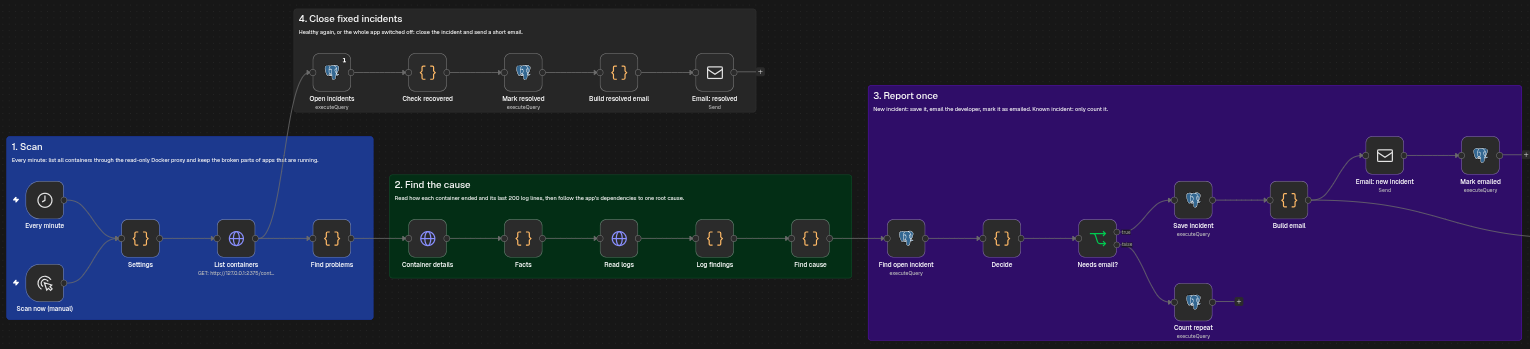
\includegraphics[width=\linewidth]{workflow-main.png}\par\vspace{0.6em}
  \raggedright\small
  \begin{columns}[T]
    \column{0.24\textwidth}\textbf{1. Scan}\par\muted{Lists all containers every minute through a read only Docker proxy}
    \column{0.24\textwidth}\textbf{2. Find the cause}\par\muted{Exit code, OOM, restarts and logs, then follows the app's dependencies}
    \column{0.24\textwidth}\textbf{3. Report once}\par\muted{Saves a new incident and emails it; known incidents are only counted}
    \column{0.24\textwidth}\textbf{4. Close}\par\muted{Healthy again: closes the incident with a short resolved email}
  \end{columns}
\end{frame}

%--------------------------------------------------
\begin{frame}{What the developer receives}
  \begin{columns}[c]
    \column{0.55\textwidth}
    \centering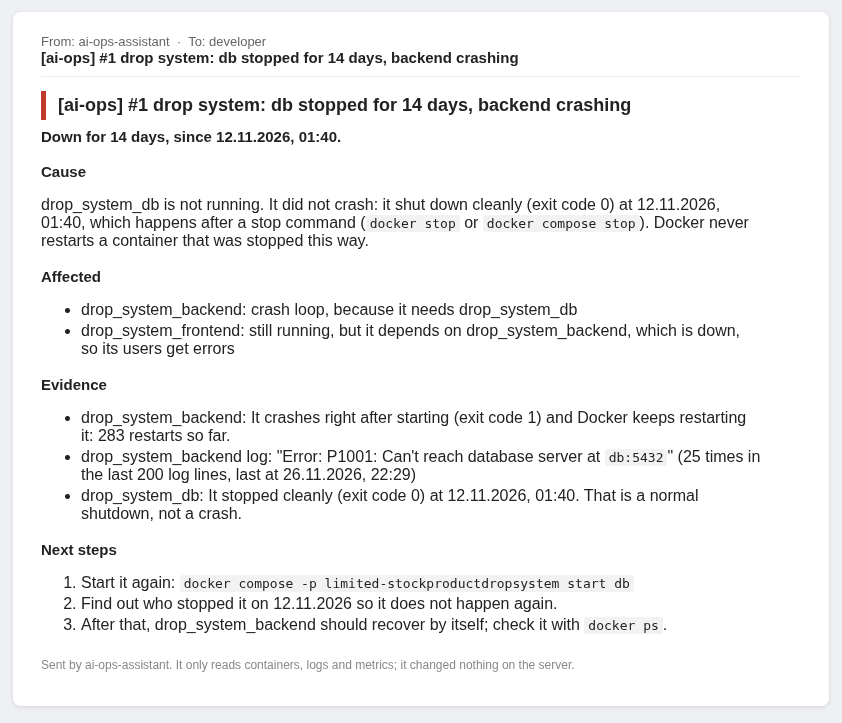
\includegraphics[height=0.78\textheight]{email-report.png}
    \column{0.4\textwidth}
    \small
    A real report from my own laptop:
    \vspace{0.5em}
    \begin{itemize}\setlength{\itemsep}{0.5em}
      \item The database of one app had been stopped for \textbf{14 days}
      \item Its backend had crashed and restarted \textbf{283 times}
      \item One email names the database as the root cause, lists the affected parts and gives the command to fix it
    \end{itemize}
  \end{columns}
\end{frame}

%--------------------------------------------------
\begin{frame}{Facts decide, not guesses}\raggedright
  \vspace{0.4em}
  \small
  \begin{tabular}{@{}>{\raggedright\arraybackslash}p{0.32\textwidth}>{\raggedright\arraybackslash}p{0.6\textwidth}@{}}
    \toprule
    \textbf{Evidence on the server} & \textbf{Cause in the report}\\
    \midrule
    Stopped container named in the logs & A dependency is down: one incident, not one per container\\
    Exit code 0, restart policy & Stopped on purpose by a command, not a crash\\
    OOMKilled, memory limit & Out of memory\\
    Error line plus stack trace & Bug in the code, with file and line\\
    EADDRINUSE, auth failed, ENOSPC & Port in use, wrong credentials, disk full\\
    \bottomrule
  \end{tabular}
  \vspace{0.9em}

  Evidence must fit the time of the event, and a container that is only waiting for its next restart is not reported as a new problem.
\end{frame}

%--------------------------------------------------
\begin{frame}{Design choices}
  \vspace{0.5em}
  \begin{columns}[T]
    \column{0.47\textwidth}
    \card{0.92\linewidth}{\textbf{Read only}\par\small\muted{The workflow reaches Docker only through a proxy that blocks start, stop and delete. Tested: a stop request returns 403.}}\par\vspace{0.6em}
    \card{0.92\linewidth}{\textbf{One email per incident}\par\small\muted{Scans run every minute, but a known problem is only counted. A failed email is sent again on the next scan.}}
    \column{0.47\textwidth}
    \card{0.92\linewidth}{\textbf{One command install}\par\small\muted{install.sh builds the n8n credentials and workflows from one .env file, imports and publishes them.}}\par\vspace{0.6em}
    \card{0.92\linewidth}{\textbf{AI only as an extra}\par\small\muted{An optional local model investigates errors the rules cannot explain. Every quote it gives is checked against real tool results.}}
  \end{columns}
\end{frame}

%--------------------------------------------------
\begin{frame}{What testing taught me}\raggedright
  \vspace{0.4em}
  \begin{itemize}\setlength{\itemsep}{0.8em}
    \item \textbf{A false alarm.} Right after a database restart, one scan read old error lines and reported a new problem. Fixed with a ``recovering'' rule and a test for each case.
    \item \textbf{A silent failure.} An incident was saved but its email failed, so it was never reported. Incidents now count as reported only after the email is sent.
    \item \textbf{The AI invented a container.} The local model answered without calling any tool and named a database that did not exist. The evidence check threw it out, and the cause stays with the rules.
    \item \textbf{16 offline tests} run the rules straight from the workflow file.
  \end{itemize}
\end{frame}

%--------------------------------------------------
\begin{frame}{Dashboard and next steps}
  \begin{columns}[c]
    \column{0.6\textwidth}
    \centering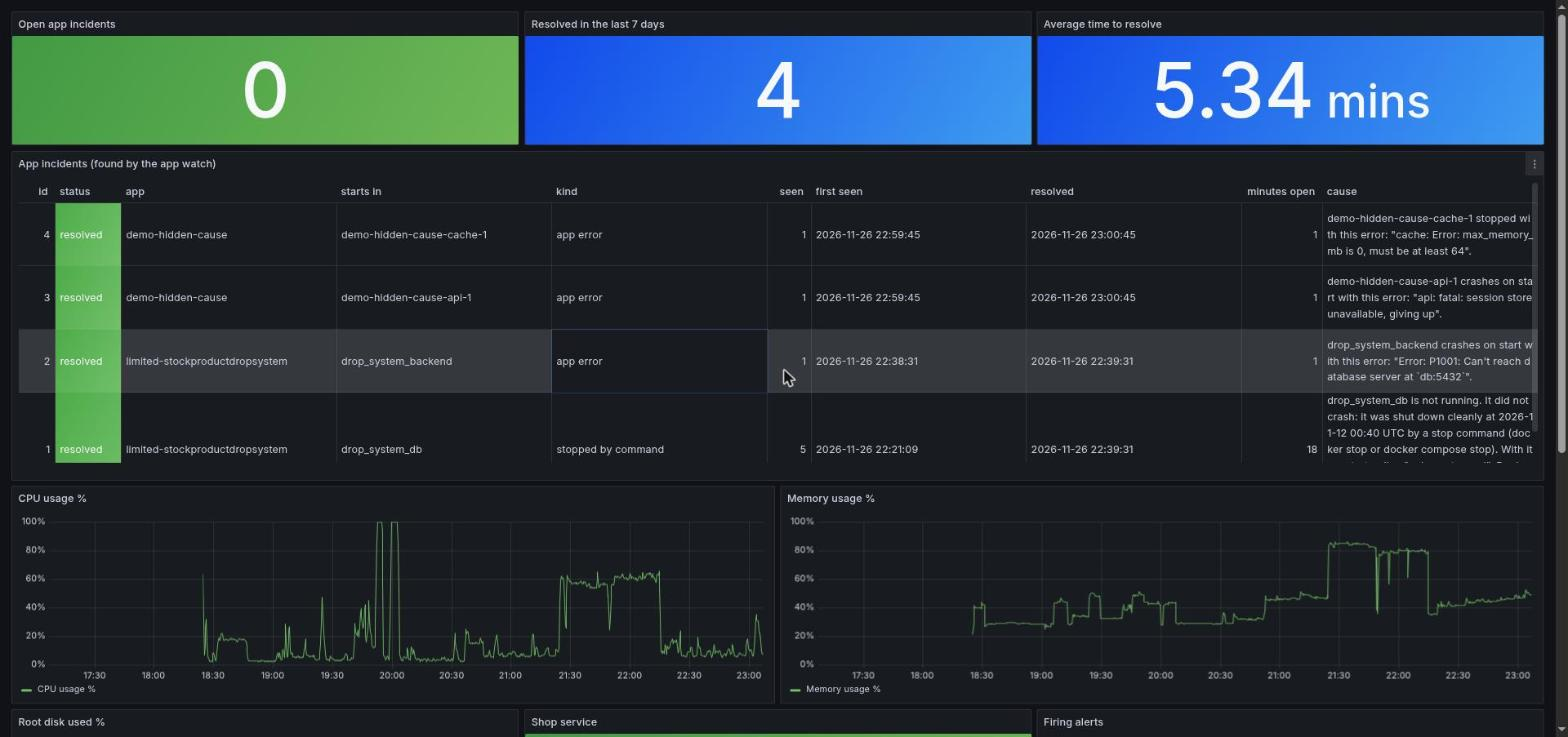
\includegraphics[width=\linewidth]{grafana-dashboard.jpg}\par
    \scriptsize\muted{Grafana: open and resolved incidents next to server health}
    \column{0.36\textwidth}
    \small\textbf{Next}
    \vspace{0.4em}
    \begin{itemize}\setlength{\itemsep}{0.5em}
      \item Run it on a live server next to a production app
      \item A heartbeat, so silence from the watcher itself is noticed
      \item Run the AI investigation on a GPU and measure it
    \end{itemize}
    \vspace{0.8em}
    {\tiny\color{muted}github.com/omar-radwan7/AI-ops-assistant}
  \end{columns}
\end{frame}

\end{document}
